\clearpage
\part{ Renderer }

\section{渲染的本质}
在渲染方面上的研究与优化已经发展成熟,已成为一个非常复杂的系统了,本文的目标是从理解渲染的技术原理,从软渲染,到CPU,再到GPU。
为简化,我们以图元三角形为例,主要有两个阶段:
\begin{itemize}
    \item {决定那些像素坐标构成这个三角形}
    \item {决定这些像素的颜色值是多少,这个过程就是着色shading}
\end{itemize}
它们分别对应着图形学中另外两个概念,光栅化和光照模型。

\subsection{光栅化Rasterize}

图形学中,是物理的三维世界,如何把三维物体在二维屏幕上显示,需要把它的三维属性都降为二维的结果,大致存在以下几个步骤:

\begin{itemize}
    \item {坐标变换}
    \item {属性计算,如颜色,纹理,alpha等}
    \item {光栅化}
\end{itemize}

目前大众屏幕分辨率为1920x1080,在二维屏幕渲染时,内存中的FrameBuffer只保存着1920x1080个屏幕点的颜色,然后再映射到屏幕上面。
光栅化的,就是计算出1920x1080个点的颜色值的过程。把物体的数学描述转换为屏幕的像素值,是从连续到离散,即物理的坐标是浮点数,而屏幕坐标是整数,光栅化的过程是一个近似的过程。
在一些图形处理软件中就是把矢量图形转化成像素点的过程。

\subsection{光照模型illumination model}
当光照射到物体表面时,物体会对光发生反射、透射、吸收、衍射、折射、干涉等。其中被物体吸收的部分转化为热。
反射、透射的光会进入人的视觉系统,使我们看见物体。为了模拟仿真这一真实的现象,建立一些数学模型来替代复杂的真实
物理模型,这些模型就称为光照模型。
\begin{itemize}
    \item {1971,Gourand提出,用漫反射模型计算多边形顶点的光亮度,再用增量法插值计算}
    \item {1975,Phong提出一个经验模型,真实度达到可以接受的程度}
    \item {1980,Whitted提出一个光透射模型,是第一个光线跟踪算法的范例,模型综合考虑了光的反射、折射、透射、阴影等,但它
    仅考虑特定方向上的环境入射光对被照射点的光亮度共线,仅能模拟理想的镜面反射和规则的投射效果}
    \item {1982,Cook和Torrance克服Phong的缺点,提出一个基于物理光学的表面反射模型-Cook-Torrance模型。使得模型中反射光
    的位置和分布与实际情况非常接近,得到画面质感很好}
    \item {1982, Blinn 体积散射}
    \item {1983,Hall和Greenbert在Whitted基础上提出Hall光透射模型,考虑了漫透射和规则透射光,改进投射高光效果,在环境
    光中加入了距离衰减因子}
    \item {1984, Cook, Porter, Carpenter 分布光线跟踪}
    \item {1986,Kajiya统一了光照模型,渲染方程,首先提出类似于随机采样的蒙特卡罗Monte Carlo方法求解绘制方程的光线追踪算法Raytracing,
    通过对达到图像平面上的光线路径进行采样,然后估计对最终图像的贡献来生成图像}
    \item {1991,Sillion的非漫射辐射度Nondiffuse radiosity}
    \item {1991, Hanrahan,分级辐射度算法Hierarchical radiosity}
    \item {1992,RenderMan规范}
    \item {1993,Lischinski,不连续网格辐射度Discontinuity meshing}
    \item {1994, 双向路径跟踪}
    \item {1995,Diffusion for light transport}
    \item {1997, 马尔科夫链蒙特卡罗}
    \item {1997,Keller的Virtual point lights(Instant Radiosity)}
    \item {1998, Jensen, Christensen, Volumetric photo mapping}
    \item {2000, Metropolis in volumes}
    \item {2001, 次表面散射}
    \item {2002,Kelemen,Primary sample space MCMC}
    \item {2005,Cline,Energy Redistribution 非遍历MCMC}
    \item {2007,Walter,Microfacet transmission model}
    \item {2008,Jarosz,光束辐射估计Beam Radiance Estimate}
    \item {2010, Jakob, Anisotropic volume media}
    \item {2011, Advanced diffusion models}
    \item {2012, Manifold Exploration}
    \item {2014, Unifying Points, Beams, and Paths}
    \item {2015, 梯度域路径跟踪}
\end{itemize}

\subsubsection{Lamertian}
1970年Bouknight提出了第一个光反射模型。1971Gourand提出“漫反射模型+插值”的思想,称为Gourand明暗处理。
即出物体表面朝向(即法线)是确定物体表面上一点光强的主要因素,用Lambert漫反射定律计算物体表面上各多
边形的光强,对光照射不到的使用环境光代替。
\textbf{Lambert's cosin law},告诉我们曲面表面的颜色c与表面法线和光源方向的夹角的余弦值cosine成正比。

\begin{math}
\begin{aligned}
c \propto cos(\theta) \\
c \propto n \cdot l 
\end{aligned}
\end{math}

漫反射:当光线从光源照射到曲面表面时,表面向每个方向散射辐射量。漫反射符合兰伯特定律。

\begin{math}
\begin{aligned}    
c_{diffuse} = max(0, \hat{n} * \hat{l}), \\
c_{ambient} = Kd * Ia, \\
c_{light} = Kd * Il, \\ 
c_{final} = c_{ambient} + c_{light}c_{diffuse}, \\
0 < Kd < 1, 
\end{aligned}
\end{math}

Kd是材质对环境光的反射系数,Ia表示环境光强度,Il表示点光源强度
注意,这里存在一个前提,就是假设光源方向l不依赖渲染物体的位置信息,就是光与渲染对象有足够的远,就是
方向光directional light。

\subsubsection{Phong Shading}
Phong模型引入镜面光,认为镜面与反射的光强盒反射光线与视线的夹角相关

\begin{figure}[h]
    \centering
    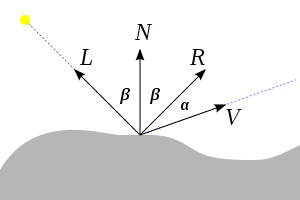
\includegraphics[width=\textwidth]{images/phong-shading-model.png}
    \caption{Phong Shading Model}
\end{figure}

图中的$\alpha$ 很小时,就是高光效果

\begin{math}
    \begin{aligned}
        R = -L + 2(L \cdot N) * N, \\
        I_{spec}=Ks * Il * (dot(V, R))^N_{s}, \\
    \end{aligned}
\end{math}

Ks为镜面反射系数,Ns为高光指数。
Blinn-Phong是基于Phong的修正模型,

\begin{math}
    \begin{aligned}
        H = \frac{L + V}{|L + V|}, \\
        I_{spec} = Ks * Il * (dot(N, H))^N_{s}
    \end{aligned}
\end{math}

H是入射光线方向L与视线方向V的中间向量,称之为半角向量。相比两者,前者更真实,后者高光更柔和,且计算速度较快,
实际中应用更广,OpenGL和DirectX渲染管线中是默认渲染模型。


\subsubsection{全局光照方程}

局部光照模型只考虑光对物体的照明,忽略了物体间的相互影响,其一般公式可以表示为

\begin{math}
    I = I_{abmient} + \sum_{i}^{N}I_{light}\frac{1}{k_{c}+k_{l} \cdot d_{i} + k_{q} \cdot d_{i}^2}
    \left[ k_{d}(N \cdot L) + k_{s}(R \cdot V)^n \right]
\end{math}

每个光源对物体的影响主要包括漫反射和镜面反射两部分,局部照明的阴影算法需要单独考虑。
\newline
全局照明考虑更全面,它自带阴影效果。它主要有两种算法:
\begin{itemize}
    \item {光线追踪法, 关注于镜面反射光,可严格追踪反射光线的方向,实际中采用逆向追踪法,减少计算量}
    \item {辐射度法, 关注于漫反射光,}
\end{itemize}
基本模型是 
\newline

\begin{math}
    \begin{aligned}
        I_r = I_{ia}R_{a} + \sum_{l}I_{il}(N \cdot L_{l})d \omega_{il}(sR_{s} + dR_{d})
    \end{aligned}
\end{math}

其中的环境光和漫反射分量不依赖于观察者的位置View's Position。假设表面是由微面元组成microfacet,其镜面分量为:
\newline

\begin{math}
    \begin{aligned}
        R_s = \frac{F}{\pi} \frac{DG}{\pi (N \cdot L)(N \cdot V)}
    \end{aligned}
\end{math}

为更加丰富,引入了几何项G,Fresnel项F,粗糙度项D。
\newline

\textbf{粗糙度项D},代表了可以有效反射光的那一部分微面元所占的比例,有多种分别函数。
高斯分布模型
\newline

\begin{math}
    \begin{aligned}
        D = ce^{-(\alpha / m)^2}
    \end{aligned}
\end{math}

Bechmann分布函数
\newline

\begin{math}
    \begin{aligned}
        D = \frac{1}{m^2cos^4(\theta)}e^-(tan\alpha / m)^2
    \end{aligned}
\end{math}

\textbf{几何项G},几何衰减项,表现了微小面元之间的互相遮挡shadowing and masking所造成的影响。
\newline

\begin{math}
    \begin{aligned}
        G = \left\{
            1, \frac{2(N \cdot H)(N \cdot V)}{(V \cdot H)}, \frac{2(N \cdot H)(N \cdot L)}{(V \cdot H)} 
        \right\}
    \end{aligned}
\end{math}

\textbf{Fresnel项F},描述了在每一个微面元上光是如何反射,与入射角和波长相关。
\newline

\begin{math}
    \begin{aligned}
        c = cos(\theta) = V \cdot H \\
        g^2 = n^2 + c^2 - 1 \\
    F = \frac{1(g-c)^2}{2(g+c)^2} \left\{ 1+\frac{[c(g+c)-1]^2}{[c(g-c)+1]^2} \right\}
    \end{aligned}
\end{math}


\subsubsection{光照类型}
目前处理光照的思路分两大类,分别是
\begin{itemize}
    \item {逐顶点光照,在每个顶点计算光照,在渲染图元内部进行插值,光照模型中的非线性关系会产生问题}
    \item {逐像素光照,Phong着色,在fragment对顶点法线进行插值}
\end{itemize}

\subsection{渲染类型}

首先从目的出发,真实感渲染与非真实感渲染NPR。

\subsubsection{Photorealistic Rendering}

真实感图形技术包括消隐技术,光照模型,明暗处理和纹理,阴影生成等

\begin{itemize}
    \item {局部光照,仅处理光源直接照射物体表面的光照模型,与光栅化渲染算法相适应的,一次只考虑
    一个像素的光照强度,逐像素的光照计算,不能得到其他像素的光照影响值}
    \begin{itemize}
        \item {Lambert漫反射模型,不能很好处理镜面与高光}
        \item {Gourand}
        \item {Phong,支持高光与镜面}
        \item {Blinn-Phong,速度快,目前商业普遍使用}
        \item {Cook-Torrance,以双向反射的基础上}
    \end{itemize}
    \item {全局光照,基于光学物理原理,光照强度的计算依赖于光能在现实世界中的传播,考虑光线与整个场景中
    各物体表面以及物体表面之间的相互影响,包括多次反射、透射、散射等,成熟应用在离线渲染中}
    \begin{itemize}
        \item {光线跟踪,模拟光从光源出发经过若干次反射、折射达到摄像机的过程,由于只有最终到达摄像机的光线
        才对生成图像有贡献,实现中是以摄像机逆向发出光线,以寻求达到光源的路径。}
        \begin{itemize}
            \item {路径跟踪Path Tracing}
            \item {递归光线追踪Whitte-type}
            \item {分布式光线追踪Distrubution}
            \item {双向路径追踪Bidirectional Path}
            \item {Metropolis}
        \end{itemize}
        \item {辐射度算法,是一种物体空间的算法,用于解离散点或环境中表面曲面面片的光强度问题,而不是解图像平面
        投影的像素问题}
        \item {光子映射,改善漫反射辉映,焦散等全局光照效果,还无法应用在实时渲染中}
    \end{itemize}
\end{itemize}

\subsubsection{Non-Photorealistic Rendering}
对于某些场景,不需要真实感,需要一些艺术化的表现
钢笔素描的生成,
中国国画与书法的生成。
\newline
\textbf{Artistic Shading},艺术渲染,模拟人简画的素描之类的,是一种根据轮廓来来抽象效果。

\subsubsection{基于图像的渲染}
Image Based Rendering,IBR。完全摒弃传统的先建模,然后确定光源的渲染方法,它直接从一系列已知的图像中生成未知
视角的图像,适用于野外极其复杂场景的生成和漫游。


\clearpage 
\section{ 算法 }

\subsection{ Edge Function }
Juan Pineda \cite{EdgeFunction} 在他论文提出的概念,就是\textbf{barycentric coordinates}的应用。
它在计算三角形属性方面上有很大的优势,如深度z-depth、颜色color、纹理坐标uv、法线等插值计算。
重心(质心)坐标的应用主要体现在:
\begin {itemize}
    \item {判断一个点是否在三角形内}
    \item {根据三角形三个顶点得到三角形内一个点P}
\end {itemize}
在软光栅化或光线追踪都用得到。

\begin{figure}[h]
    \centering
    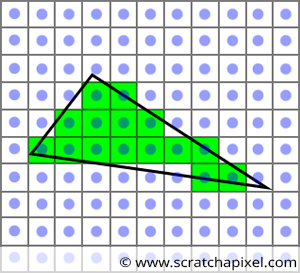
\includegraphics[width=0.25\textwidth]{images/rasterization-triangle1}
    \hspace{0.1cm}
    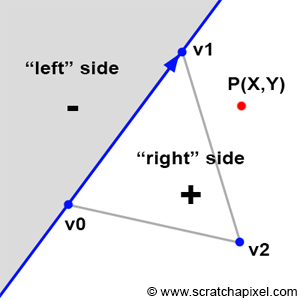
\includegraphics[width=0.25\textwidth]{images/rasterization-triangle2}
    \hspace{0.1cm}
    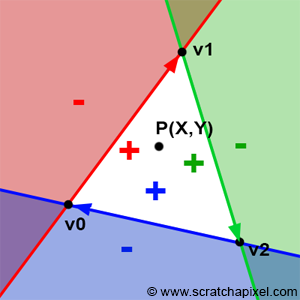
\includegraphics[width=0.25\textwidth]{images/rasterization-triangle3}
    \caption{左边:测试像素是否覆盖三角形,是光栅化算法的原理;
    中间:判断点与线的关系,大于0在右边,小于0在左边,等于0在线上;
    右边:在白色区域中的点都是位于三角形边的右边
    }    
\end{figure}
遍历整个FrameBuffer去判断点是不是在在三角形内部,太浪费时间去遍历不可能的结果了。
\begin{figure}[h]
    \centering
    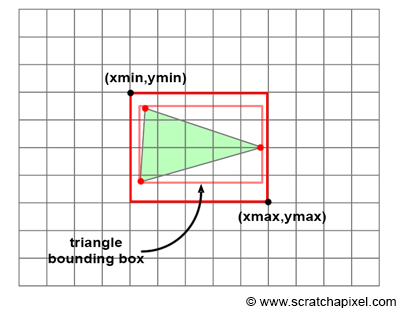
\includegraphics[width=0.3\textwidth]{images/rasterization-boundingbox.png}
    \caption {三角形的顶点告诉了大致范围,减少遍历的次数,提高访问性能}
\end{figure}
计算boundingbox的算法很简单,速度也快。

\subsection{Reconstructing Position From Depth}
需求:根据当前像素的Depth计算出View空间中的Position
先分析depth是如何计算出来的,在vertex shadeer中
\begin{lstlisting}
    outPos = mul(inPos, mvp);
    outDepth.xy = outPos.zw;
\end{lstlisting}
在pixel shader中,
\begin{lstlisting}
    depth = outDepth.x / outDepth.y;
\end{lstlisting}
按照这个过程逆运算回去
\begin{lstlisting}
    z = texture(depthSampler, inUV);
    x = inUV.x * 2 - 1;
    y = (1 - inUV.y) * 2 - 1;
    pos = (x,y,z,1)
    pos = mul(pos, mvpInverse);
    pos = pos.xyz / pos.w;
\end{lstlisting}
但是存在一些问题
\begin{itemize}
    \item {z/w是非线性分布的,经过RTT(Render To Texture)后再变换回去,精度存在误差}
    \item {计算量大}
\end{itemize}
从物理状态来看看摄像机的视锥体的抽象形式,从摄像机位置到远裁剪面发射一条射线,存在一个关系:

\begin{figure}[h]
    \centering
    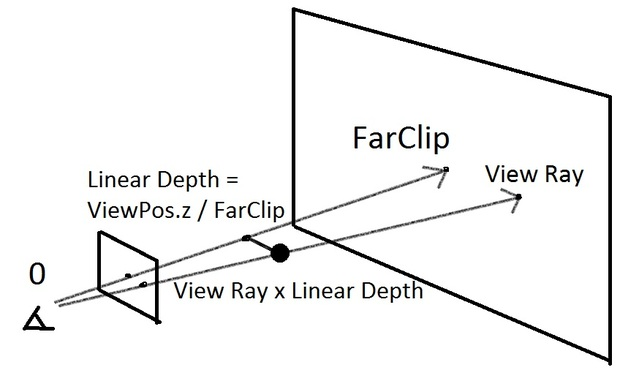
\includegraphics[width=0.5\textwidth]{images/reconstructing-position-from-depth.png}
\end{figure}

\begin{lstlisting}
    posView = viewRayDir * linearDepth;    
    linearDepth = posView.z / farClipDistance;
\end{lstlisting}

linearDepth是规格化的Z值,它满足线性分布。现在的问题就如何得到RayDir向量了。在View空间中,摄像机的位置是(0,0,0),
对于可见的每个点,从摄像机出发的射线都与远裁剪面相交,交点就是方向向量RayDir的坐标。由图中可知,是利用中心线和射线组成的三角形,满足等比关系,是线性关系。
远裁剪面的四个顶点是可以计算出来的,思路就出来了。

\begin{itemize}
    \item {1. 把posView.z/farClipDistance的值保存到RTT中,得到的值满足线性关系}
    \item {2. 从RTT中得到linearDepth, 从vertex shader中得到viewRayDire.xy, }
\end{itemize}

\begin{lstlisting}
    viewRayDir = float3(farClip.x, farClip.y, farClipDistance);
    posView = viewRayDir * linearDepth;
\end{lstlisting}

\subsection{Trackball}
轨迹球\cite{Trackball}
轨迹球就是在屏幕之外虚构一个球形曲面,使鼠标在二维屏幕上的移动投影到球形曲面上。
即一个半球覆盖在屏幕上面。以屏幕中心为球心O,X轴向右,Y轴向上,Z轴向外。当鼠标在球面的范围内移动时,可以由二维屏幕上的二维左边点P(x,y),通过数学关系求得其在球面上的投影点P'。
鼠标从P1移动到P2,对应的球面就是从P1'到P2'。产生两个向量V1=OP1',V2=OP2',  
V1与V2的叉乘得到向量N,即三维物体的旋转轴,V1到V2的转角量就是三维物体的旋转角度。
屏幕时矩形,球形的投影在屏幕的平面上只会是一个圆,总会有些区域的点投影后会落在球面之外。

\subsection{Camera}

关于camera的自动对焦算法,对透视camera有: side是bounding box的最大边, distance是从camera的位置到bounding box的中心距离

\begin{math}
    tan(\alpha / 2) = (side / 2) / distance
\end{math}

对应的threejs的代码如下:

\begin{lstlisting}
    let box = calculateBoundingBoxInScene();
    let center = new THREE.Vector3(), size = new THREE.Vector3();
    box.getCenter(center); box.getSize(size);
    let maxSide = Math.max(size.x, Math.max(size.y, size.z));    
    let distance = maxSide /
         ( 2 * Math.tan(THREE.Math.DEG2RAD * alpha / 2));  
    camera.position.set(center.x, center.y, center.z - distance);
    camera.position.z *= Math.sqrt(3);
\end{lstlisting}




\clearpage
\section{线性变换}


线性变换主要包括缩放、旋转、反射等,不包含平移。线性变换的数学描述为:

\begin{math}
\begin{aligned}
f(\alpha v)=\alpha v, \\
f(u+v)=f(u)+f(v)
\end{aligned}
\end{math}

反射,就是把一个物体变换成它的镜像的映射,在二维空间中,用一条直线作为“镜子”;在三维空间中,使用平面作为“镜子”。

\subsection{ 坐标coordinate}

\subsubsection{重心坐标}
barycentric coordinate.


\subsection{ 矩阵matrix }
矩阵就是线性变换
\subsubsection{特征向量eigenvector}
对于一个给定的线性变换(矩阵M,是向量空间E到自身的一个线性变换,可以旋转、反射、拉伸、压缩或变换的组合),它的特征向量V经过这个线性变换之后,得到新的向量U,VU向量共线,但长度可能不一致。
VU的长度缩放的比例称为特征值eigenvalue。

\subsubsection{余子式minor}
在n阶行列式D中划去任意选定的k行、k列后,余下的元素按照原来的顺序组成的n-k阶行列式M,M称为
行列式D的k阶子式A的余子式Minor。如果k阶子式A在行列式D中的行和列的标号分别为
$i_{1},i_{2},...,i_{k}$和$j_{1},j_{2},...,j_{k}$。则在A的余子式M前面加一个符号:
\begin{math}
    \begin{aligned}
        {-1}^{(i_{1}+i_{2}+...+i_{k}) + (j_{1}+j_{2}+...+j_{k})}
    \end{aligned}
\end{math}
得到的n-k阶行列式,称为行列式D的k阶子式A的代数余子式Cofactor。

\subsubsection{行列式determinant}
行列式其实是一个函数,一个将方阵转换成一个标量的函数。行列式可以看做是有向面积的概念在一般的欧几里得空间中的推广。
行列式表示的是线性变换前后的面积(二维)、(三维为体积)等变化的系数。

n阶行列式det(D)等于其任意行(列)的元素与对应的代数余子式的乘积之和。通过D的i行row来计算

\begin{math}
    \begin{aligned}
   \det(D)=d_{i1}A_{i1}+...+d_{in}A_{in}=\sum_{j=1}^{n}{a_{ij}(-1)^{(i+j)}A_{ij}}
    \end{aligned}
\end{math}

又称为拉普拉斯展开式Laplace expansion,或代数余子式展开式Cofactor expansion
矩阵和行列式是两个完全不一样的概念,行列式的行和列必须相等。

\subsubsection{伴随矩阵adjoint matrix}
行列式D的每个元素的代数余子式$A_{ij}$所构成的矩阵,称为矩阵D的伴随矩阵。

\begin{math}
    \begin{aligned}
A^{*}= \begin{pmatrix} A_{11}&A_{21}&A_{...}&A_{n1} \\
A_{12}&A_{22}&A_{...}&A_{n2} \\
A_{...}&A_{...}&A_{...}&A_{...} \\
A_{1n}&A_{2n}&A_{...}&A_{nn} \end{pmatrix} = (A_{ij})^T
\end{aligned}
\end{math}

伴随矩阵就是线性变换的逆操作,再进行一个缩放的结果,缩放的大小与矩阵的行列式的值有关。
伴随矩阵定理:
A是n阶方阵,$A^*$是A的伴随矩阵,则有$AA^*=A^*A=AE$。

\subsubsection{逆矩阵inverse matrix}
n阶方阵A,存在n阶方阵B,满足$AB=BA=E$,称方阵A可逆,称方阵B是A的逆矩阵,记为$B=A^{-1}$

由伴随矩阵定理与逆矩阵可得

\begin{math}
    \begin{aligned}
\begin{cases} A^*A=E\\ AA*=|A|E \end{cases} \Rightarrow A^{-1}=\frac{A^*}{|A|}
\end{aligned}
\end{math}


\subsubsection{正交矩阵}
两个向量的内积为零,就说这两个向量是正交的,在三维空间中,正交的两个向量相互垂直。如果相互正交
向量的长度均为1,又叫做标准正交基。
在矩阵论中,\textbf{实数}正交矩阵是方块矩阵Q,它的转置矩阵是它的逆矩阵,$Q^TQ=QQ^T=I$。
注意实数二字,正交矩阵中的元素都是实数,包含复数并且同样满足正交性质的矩阵是酉矩阵,也就是推广
到复数域之后的“正交矩阵”。

\subsubsection{相似矩阵}
两个n阶方阵矩阵A与B为相似矩阵当且仅当存在一个n阶方阵的可逆矩阵P,使得$P^{-1}AP=B$或$AP=PB$,
P被称为矩阵A与B之间的相似变换矩阵。
白话就是,矩阵是线性空间中的线性变换的一个描述,在一个线性空间中,只要我们选定一组基,那么对于
任何一个线性变换,都能够用一个确定的矩阵来加以描述。同样的,对于一个线性变换,只要逆选定一组基,
那么就可以找到一个矩阵来描述这个线性变换。换一组基,就得到一个不同的矩阵。所有这些矩阵都是这
同一个线性变换的描述,但又都不是线性变换本身。所有这些同一个线性变换的描述的矩阵互为\textbf{相似矩阵}。

\subsubsection{过渡矩阵}
transition matrix过渡矩阵这个词在数学语境中有很多地方用得,在线性代数中,它用来表示坐标矩阵的变换。
\newline
设V为n维向量空间,有两个基$S=\{v_1,...,v_n\}$和$T=\{w_1,...,w_n\}$,
过渡矩阵$P_{S \leftarrow T}$从T到S的nxn矩阵,它的列项在基S中的形式为:

\begin{math}
    P_{S \rightarrow T} = [[w_1]_S [w_2]_S ... [w_n]_S]
\end{math}

举例说明:设$S=\{ e_1,e_2,e_3\}$为标准基,$T=\{ w_1=\begin{bmatrix} 1\\ 1\\ 0 \end{bmatrix}\quad, w_2=\begin{bmatrix}0\\1\\2\end{bmatrix}\quad 
, w_3=\begin{bmatrix} 1\\1\\1 \end{bmatrix}\quad \}$。

则有\newline
$P_{S \leftarrow T}=\begin{bmatrix} 1&0&1\\1&1&1\\0&2&1\end{bmatrix}$。

根据这个关系,可以表示$w_3=2e_2+e_3$。

具体数值的例子:设$S=\{ v_1=\begin{bmatrix}1\\2\\3\end{bmatrix}\quad, v_2=\begin{bmatrix}-2\\1\\0\end{bmatrix}\quad 
, v_3=\begin{bmatrix} 1\\0\\1 \end{bmatrix}\quad \}$, $T=\{ w_1=\begin{bmatrix} 1\\1\\0\end{bmatrix}\quad, w_2=\begin{bmatrix}0\\1\\2\end{bmatrix}\quad 
, w_3=\begin{bmatrix} 1\\1\\1 \end{bmatrix}\quad \}$。

求得在基S中的$w_1$的坐标值$x_1,x_2,x_3$。
\newline
由线性关系可得

\begin{math}
    x_1v_1+x_2v_2+x_3v_3=w_1
\end{math}

它的增广矩阵为
\begin{math}
    [ { \begin{array}{c:c:c:c} 
        \begin{matrix} v_1&v_2&v_3 \end{matrix} &
        \begin{matrix} w_1 \end{matrix} &
        \begin{matrix} w_2 \end{matrix} &
        \begin{matrix} w_3 \end{matrix} 
    \end{array}} ] = \Bigg [ {\begin{array}{c:c:c:c} 
        \begin{matrix} 1&-2&1\\2&1&0\\3&0&1 \end{matrix} &
        \begin{matrix} 1\\1\\0 \end{matrix} &
        \begin{matrix} 0\\1\\2 \end{matrix} &
        \begin{matrix} 1\\1\\1 \end{matrix} 
    \end{array}}
    \Bigg ]
\end{math}

对增广矩阵化简得到
\begin{math}
    \Bigg [ {\begin{array}{c:c:c:c} 
    \begin{matrix} 1&0&0\\0&1&0\\0&0&1 \end{matrix} &
    \begin{matrix} 1.5\\-2\\-4.5 \end{matrix} &
    \begin{matrix} 0\\1\\2 \end{matrix} &
    \begin{matrix} 1\\-1\\-2 \end{matrix} 
\end{array}}
\Bigg ]
\end{math}

得到的最后三列就是$[w_1]_S, [w_2]_S,[w_3]_S$, 即过渡矩阵为
\begin{math}
    P_{S \leftarrow T} = \begin{bmatrix}
        1.5 & 0 & 1 \\
        -2 & 1 & -1 \\
        -4.5 & 2 & 2
    \end{bmatrix}
\end{math}

过渡矩阵应用在:骨骼算法中,
